% -*- coding: utf-8 -*-
\newpage
\section{Topological Analysis}

The topological analysis, involving the identification of \glspl{CP} and the
evaluation of their properties, constitutes the first step in any \gls{QTAIM}
analysis. This procedure is carried out whenever the \gls{QTAIM} block is
included in the run script, and is essential for subsequent analyses.  It is
therefore mandatory for all \texttt{AnalysisLevel} settings, which may enclose
atomic as well as non-local properties, with each stage computed only after the
previous level, from topological to atomic to non-local properties.

\begin{lstlisting}[language=bash]
  QTAIM
    # [topological analysis / atomic properties / non-local properties]
    AnalysisLevel [Normal/Extended/Full]
  End
\end{lstlisting}

\subsection{Non-Nuclear Attractors (\glspl{NNA})}

Nuclear attractors are added to the array of \glspl{CP} before initiating the
search for other \glspl{CP}. Their properties are evaluated after applying a
small displacement to the nuclear coordinates ($10^{-8}$~bohr) to prevent
numerical instabilities in the evaluation of the electron density at the
nuclear positions.

A Newton-Raphson algorithm is then used to locate the remaining \glspl{CP} of
$\rho(\mathbf{r})$, which are classified according to their eigenvalue
signatures. In earlier versions of the code, \glspl{NNA} could be identified
from this signature, but no dedicated treatment was implemented; such points
were simply ignored in subsequent property calculations.

In the current implementation, \glspl{NNA} are explicitly recognised, labelled,
and fully incorporated into the analysis. All available properties are computed
for them, and they are considered on the same footing as nuclear attractors,
including their possible participation in bonds, rings, and cages.

Whenever one or more \glspl{NNA} are detected, the global variable storing the
\texttt{xyz} coordinates of the attractors is extended to include them, and the
global counter for the number of attractors is updated accordingly. These
variables are used throughout \ams code for the \gls{QTAIM} partition,
whereas in other parts of \ams the atom count continues to exclude
\glspl{NNA}.

\newpage
\vspace*{1.5cm}%
% -*- coding: utf-8 -*-
\begin{algorithm}[h!]
  \SetNoFillComment

  ncp $\gets$ natoms \tcp*{Initialise number of critical points}
  nattractors $\gets$ natoms \tcp*{Initialise number of attractors}

  \tcc{cpResults is an array to store the Results of every CP}
  % \For{iAtom \textbf{in} natoms}{
  \For{$iAtom \gets 1$ \KwTo $natoms$}{
     shiftedCoord = xyznuc(iAtom) + smallShift \tcp*{10\^{}-8}
     CalcDensity(shiftedCoord, rho, gradRho, secDerRho)\;
     cpResult(iAtom, coords) $\gets$ xyznuc(iAtom)\;
     cpResult(iAtom, density) $\gets$ rho\;
     cpResult(iAtom, gradeent) $\gets$ gradRho\;
     cpResult(iAtom, hessian) $\gets$ secDerRho\;
     cpResult(iAtom, sisnature) $\gets$ 1.0 \tcp*{Nuclear critical point}
  }

  FindAllCriticalPoints()\;

  \tcc{CharacterizeCriticalPoints}
  \tcc{ncp is the number of critical points found}
  \For{ipoint $\gets 1$ \KwTo ncp}{
    hessian $\gets$ symmetricMatrix(cpResult(ipoint, idxHessian:idxHessian+5))\;
    \tcc{LAPACK subroutine for eigenvalues of symmetric matrices}
    eigenvalues $\gets$ dsyev(hessian)\;
    signature $\gets$ DetermineCPSignature(eigenvalues)\;

    \uIf{signature == $2$}{
      ncages $\gets$ ncages + 1 \tcp*{Cage CP; All eigenvalues negative}
    }
    \uIf{signature == $3$}{
      nbonds $\gets$ nbonds + 1 \tcp*{Bond CP; Two eigenvalues negative}
    }
    \uIf{signature == $4$}{
      nrings $\gets$ nrings + 1 \tcp*{Ring CP; One eigenvalue negative}
    }
    \uIf{signature == $1$}{
      nattractors $\gets$ nattractors + 1 \tcp*{Attractor CP; All egienvalues positive}
    }
  }

  \uIf{nattractors > natoms}{
    UpdateGlobalVariablesForQTAIM()\;
  }

  \caption{\gls{NNA} treatment.}
  \label{algonna}
\end{algorithm}


\newpage

\subsection{Poincaré-Hopf relation}

The original implementation already included an evaluation of the
Poincar´-Hopf relation. In the current version of the code, its role has been
extended beyond a simple check, serving as a robust criterion for verifying
whether all \glspl{CP} in the system have been correctly identified. The
Poincaré-Hopf relation states that the sum of the indices of all \glspl{CP}
must be equal to either~0 or~1, depending on the topological nature of the
system (as discussed in Section~\ref{phsection}). This property arises from the
topology of vector fields and provides an elegant and efficient global
consistency check.

For closed systems, the expected sum is~1, whereas for
periodic systems it is~0. Since \ams is capable of treating both classes of
systems ---\adf and \dftb for molecular calculations, and \band for periodic
ones--- the implementation must account for both possibilities, as
written in the Equation~\ref{phCriterion}.

% coarser
In practice, this criterion is used to determine whether the search for
\glspl{CP} should be repeated with a finer spatial grid. When the
relation is not satisfied, the grid spacing can be reduced by factors of~2 or~3
to increase resolution, improving the likelihood of detecting missing
\glspl{CP}. Conversely, if the initial spacing is unnecessarily fine, it may be
enlarged by a factor of~2 to decrease memory requirements and avoid potential
\overflow\ errors. This adaptive refinement strategy provides a balance between
numerical accuracy and computational efficiency, ensuring reliable results
across a wide range of systems.

\begin{align}
  \chi(M) =
  \begin{cases}
    (n_{\text{NNACP}} + n_{\text{NCP}}) - n_{\text{BCP}} + n_{\text{RCP}} - n_{\text{CCP}} &= 1 \quad molecular\\
    (n_{\text{NNACP}} + n_{\text{NCP}}) - n_{\text{BCP}} + n_{\text{RCP}} - n_{\text{CCP}} &= 0 \quad periodic
  \end{cases}
  \label{phCriterion}
\end{align}

\newpage
\vspace*{1.5cm}%
% -*- coding: utf-8 -*-
\begin{algorithm}[h]
  \SetNoFillComment

  \tcc{total energy subroutine calls AIMCriticalPoints}

  \tcc{AIMCriticalPoints looks like this:}
  gridRefinements $\gets$ [1.0, 0.5, 0.66] \tcp*{Grid refinement factors}
  gross $\gets$ 1.0 \tcp*{Inflation factor in case of overflow}
  poincaréHopfTarget $\gets$ [0 or 1] \tcp*{Periodic or Molecular system}

  gridSpacing $\gets$ user-defined or default (0.5)\;  
  igrid $\gets$ 1\;
  belowOverflow $\gets$ true; everythingTried $\gets$ false; success $\gets$ false\;
  \While {belowOverflow \textbf{and} \textbf{not} success \textbf{and} igrid $\leq$ length(gridRefinements)}{

    \tcc{Update grid spacing using gridRefinements[igrid] and gross}
    gridSpacing $\gets$ gridSpacing*gridRefinements[igrid]*gross\;

    \If{igrid $>$ 1}{
      Notify(`Refining grid...')
    }

    \If{grid causes overflow}{
      Notify(`Grid too small; trying gross grid')\;
      gross $\gets$ 2.0\;
    }

    FindCriticalPoints()\;
    ClassifyCriticalPoints()\;

    \If{periodic}{
      Generate equivalent CPs\tcp*{BAND}
    }

    success $\gets$ CheckPoincaréHopf()\;
    \uIf {success}{
      \textbf{break}\;
    }
    igrid $\gets$ igrid + 1\;
  }

  \caption{AIMCriticalPoints Subroutine}
  \label{grid_refinement}
\end{algorithm}



\newpage
\subsection{Bonds, Rings and Cages}

Once all \glspl{CP} have been successfully identified, the next step is
to determine the atoms involved in bonds, rings, and cages. In earlier
versions of the code, only atoms in bonds could be identified, with no
support for detecting ring or cage structures.

The identification of atoms involved in bonds, rings and cages is performed by
following the gradient path with the corresponding \gls{CP} as starting point. For bonds, the
number of atoms and the directions to follow the gradient path are already known, two
atoms and the directios are given the third eigenvector in both the positive
and negative directions. In contrast, for rings and cages, neither the number
of atoms nor the optimal directions for following the gradient path are known
in advance.

To address this, we construct a spherical shell (icosphere) of points around
the \gls{RCP} or \gls{CCP} and follow the gradient path from each point. The
choice of the shell radius is critical: if it is too small, many points follow
nearly identical paths and fail to reach all atoms; if too large, the
integration path may overshoot the ring or cage. Further details on the
generation of the icosphere are provided in Appendix~\ref{icosphereGeo}.

\begin{figure}[h!]
  \centering
  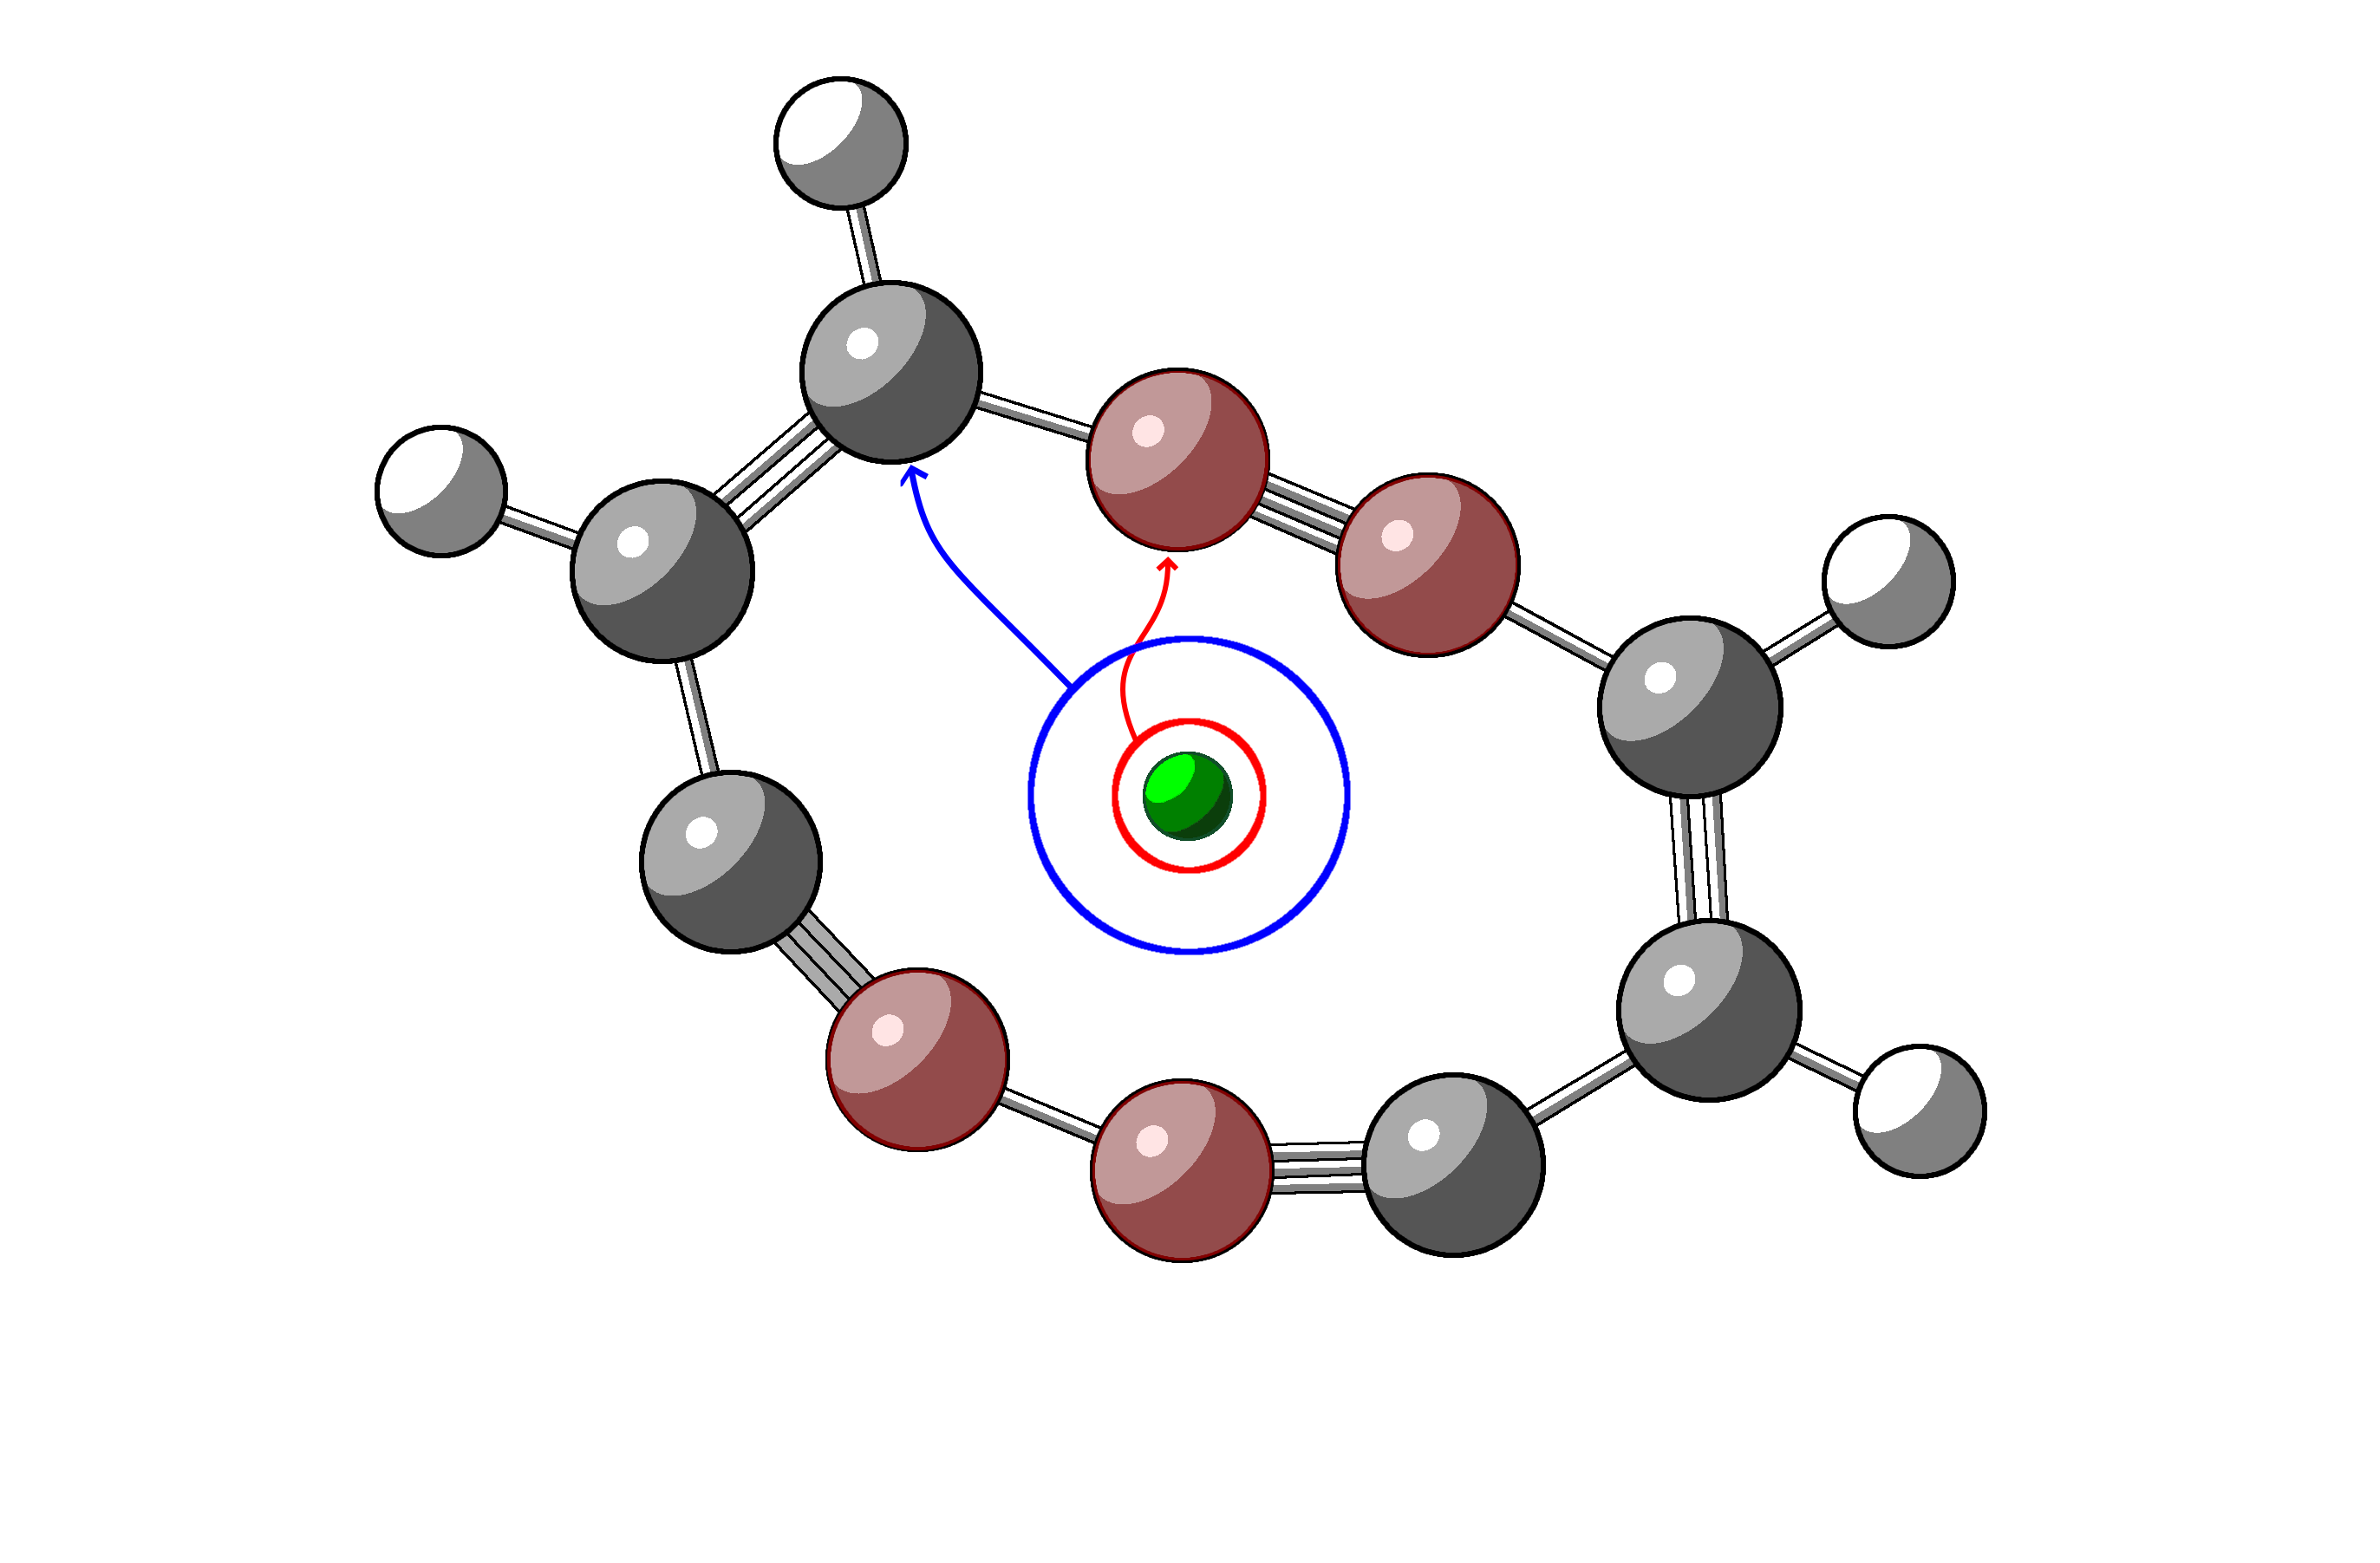
\includegraphics[width=0.85\textwidth]{img/c10_cartoon.png}
  \caption{The \gls{RCP} (green sphere) is enclosed by two icospheres: a red
    one (0.2~bohr) and a blue one (0.6~bohr). Gradient paths originating from the
    red icosphere reach only the atoms highlighted in red, whereas those from the
    blue icosphere connect to all atoms in the ring. For each case, one
    representative gradient path is shown.}
  \label{c10}
\end{figure}

\newpage
The radius must be sufficiently small to capture compact structures such
as cyclopropene. A value of 0.2~bohr has been found to work reliably in
such cases. For more distorted rings, or those closed by non-covalent
interactions, larger radii are required. We have therefore implemented
three radii (0.2, 0.6, and 2.8~bohr) to accommodate a range of
geometries. As illustrated in Figure~\ref{c10}, a radius of 0.2~bohr may
fail to detect all atoms in very flat density regions, where gradient
paths initiated from similar directions converge. A larger radius allows
paths to explore the full structure more effectively.

The accuracy of the differential equation solver plays a decisive role in
correctly following the gradient paths. By default, a second-order Runge-Kutta
method is used. If the initial search fails to identify valid paths, the solver
is automatically upgraded to a fourth-order Runge-Kutta method.

Finally, for each bond, ring, and cage \gls{CP}, the set of atoms assigned to
the corresponding structure is verified to contain only unique entries. In
systems characterised by extremely flat electron densities, it is possible for
multiple gradient paths to converge on the same attractor, \eg a bond cannot be
formed by the same atom twice.

\vspace{0.7cm}%
\subsection{Graph theory}

In the previous section, we described the attempts to follow gradient
paths from \glspl{RCP} and \glspl{CCP}. Here, we explain how the program
determines whether recomputation of these paths is necessary. This is
achieved through a graph theory analysis, it is used to validate if the
topological features have been correctly identified.

For rings, we require that the number of atoms equals the number of
bonds, and that each atom forms exactly two bonds with the other ring
atoms. These simple criteria allow us to confirm the topology. If either
condition is not met, the gradient paths are recomputed using a smaller
step size and a higher-order Runge-Kutta method.

\newpage

\begin{wrapfigure}[12]{o}{0.47\textwidth}% Add about AIMAll
  \centering
  \vspace*{-0.5cm}%
  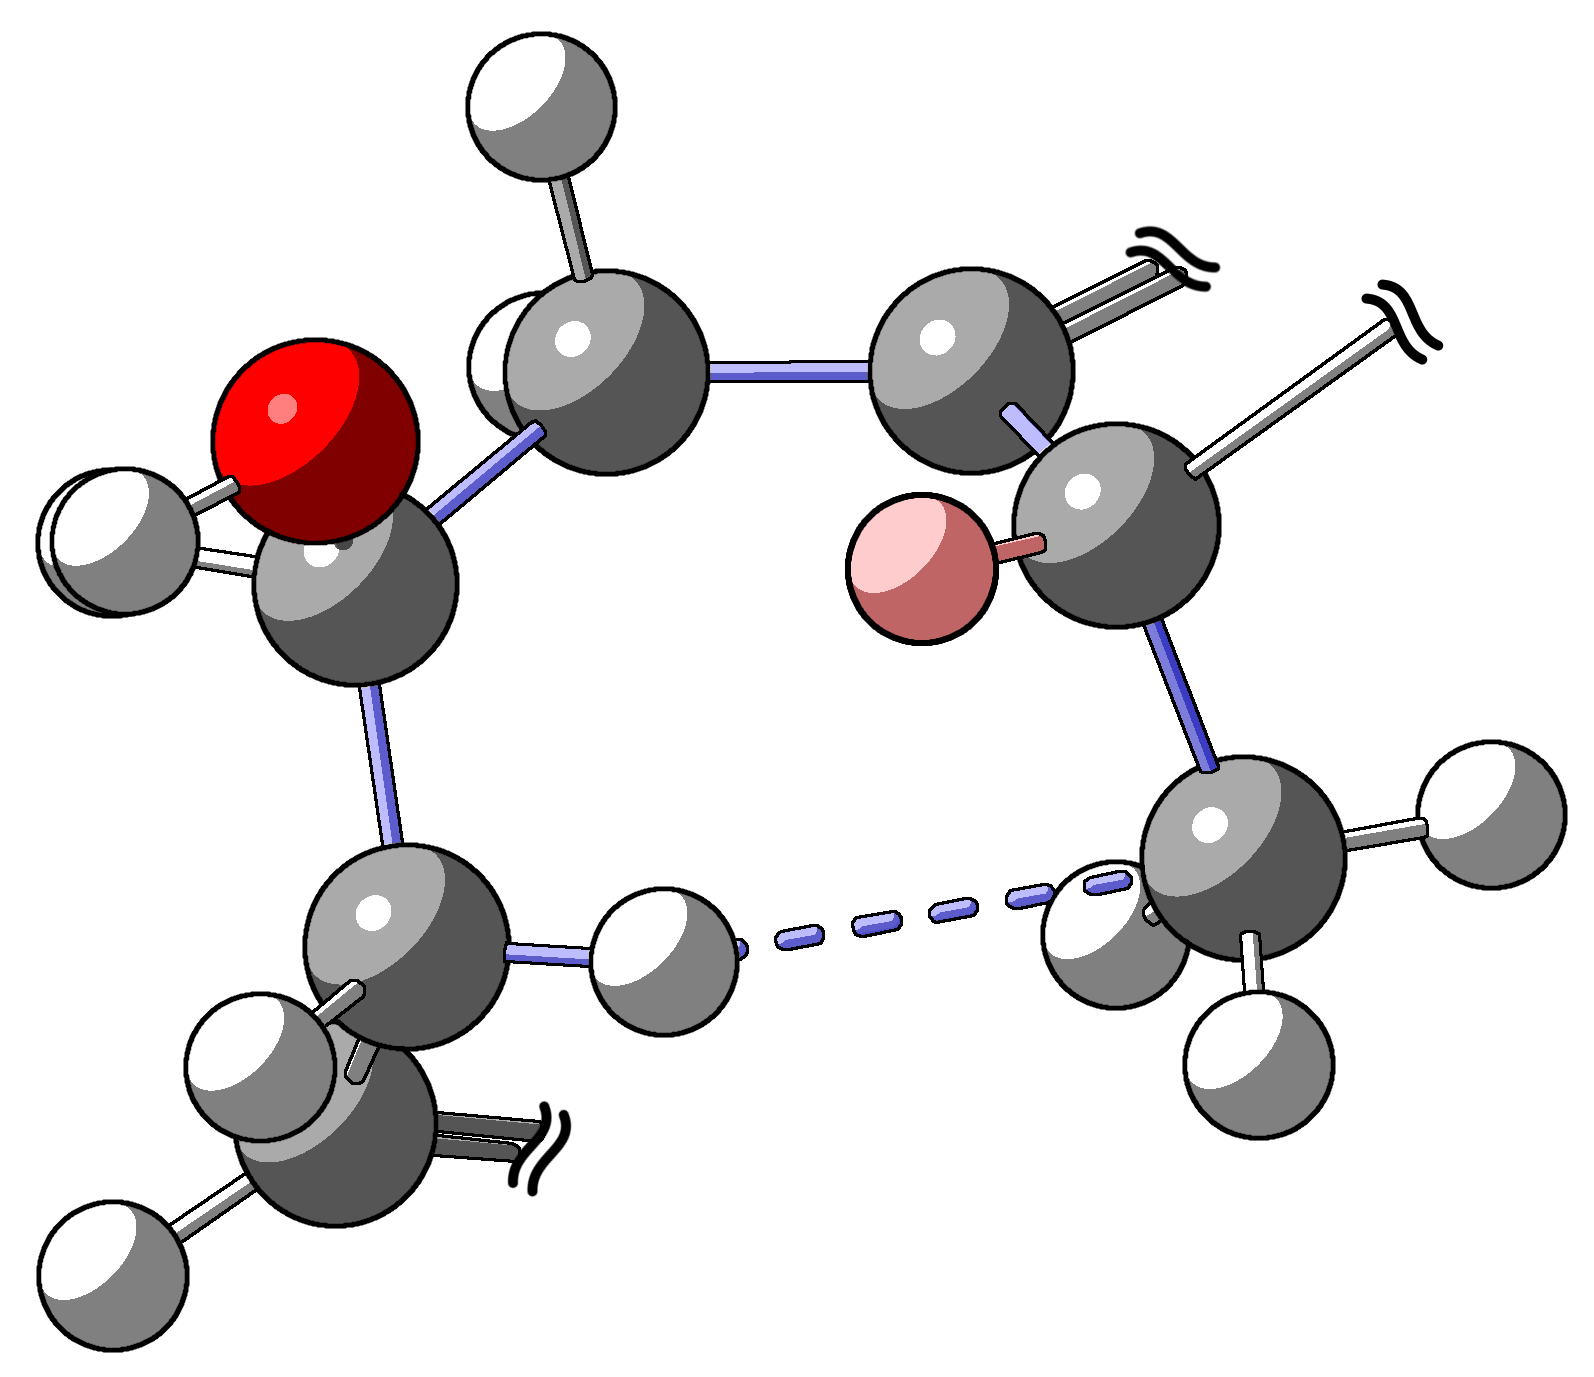
\includegraphics[width=0.47\textwidth]{img/extra_atom.png}
  \caption{Extra H atom highlighted in pink detected in a ring. Parts
    of the molecule are
    ommited for clarity. The \texttt{xyz} coordinates
    are available in the Appendix~\ref{xyzfiles}.}
  \label{extra_atom}
\end{wrapfigure}

\vspace*{0.1cm}%
In one particular case the recomputation can be avoided. If exactly one extra
atom is detected in a ring, it is likely an artefact. As shown in
Figure~\ref{extra_atom}, a hydrogen atom close to the ring plane may be
erroneously assigned to the ring when following the gradient path. Computing
the system's topology with \aimall, we observe the misassignment of the H atom
to the ring as an artefact of following the gradient path. Such atoms can be
excluded from the final ring definition to prevent unnecessary recomputation.

\vspace*{0.8cm}%
If, after all tries, the topology remains inconsistent, a warning is issued in
the output file. In the case of cages, even exotic topologies can be valid
topologies. We therefore avoid rigid definitions, choosing instead to alert the
user to atypical situations.

For rings, in case that the atoms does not form a valid cycle, we issue the
warning:
$i$) not all atoms in a ring have been successfully identified.
%
% \begin{itemize}[itemsep=0.01em]
% \item[$i$)] not all atoms in a ring have been successfully identified.
% \end{itemize}
While for cages, we issue the following warnings for potentially non-standard
topologies:
%
\begin{itemize}[itemsep=0.0em]
  \item[$i$)] a bond associated with a cage does not belong to at least two rings,
  \item[$ii$)] not all atoms in a cage have at least three bonds,
  \item[$iii$)] a cage is not a convex polyhedron,
  \item[$iv$)] a cage and at least one ring are composed of the same atoms,
  \item[$v$)] all atoms in a cage are also in a ring that contains additional atoms.
\end{itemize}

\newpage
\begin{wrapfigure}[10]{o}{0.5\textwidth}
  \centering
  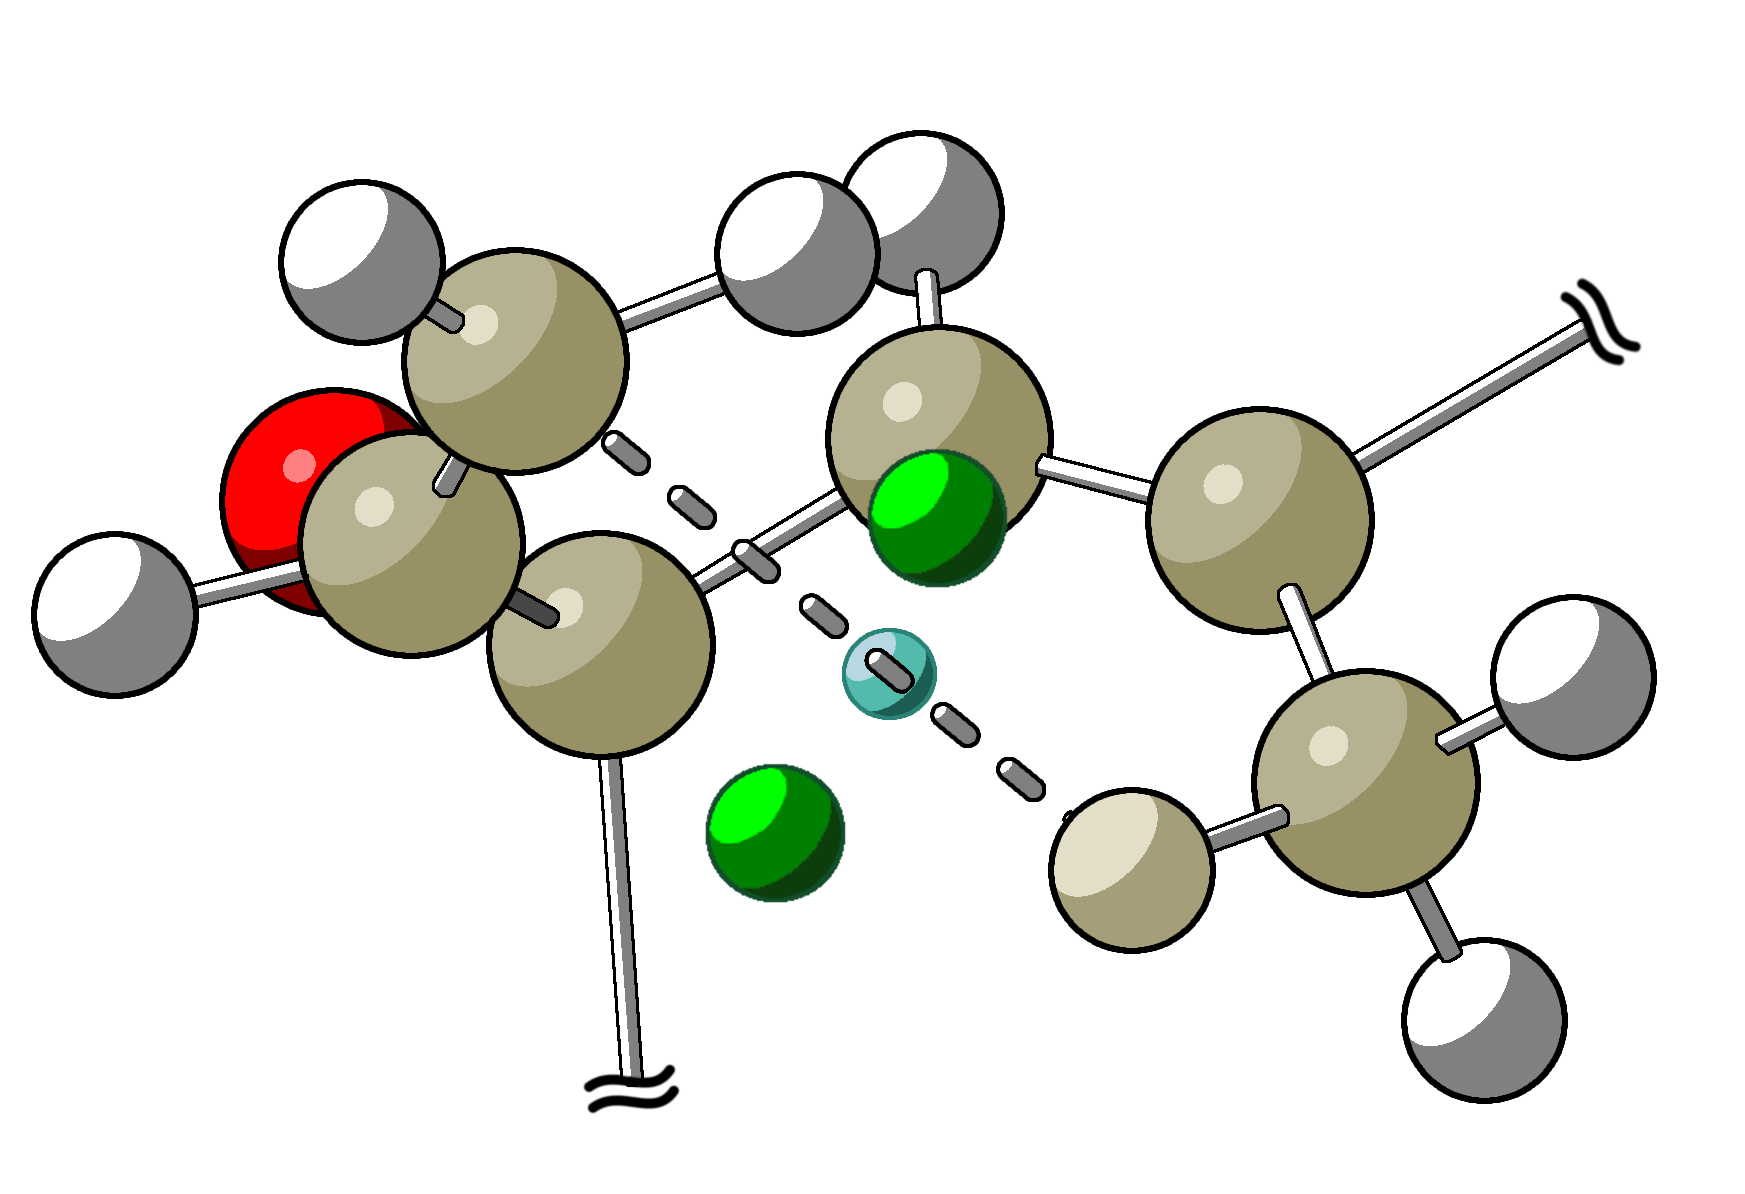
\includegraphics[width=0.5\textwidth]{img/ring_cage}
  \caption{Cage formed by two rings. The two \glspl{RCP} (green spheres) share
    the same atoms (highlighted in khaki), creating the \gls{CCP} (blue sphere).
    Parts of the molecule are omitted for clarity. The atomic coordinates are
    available in the Appendix~\ref{xyzfiles}.}
  \label{cage_extra}
\end{wrapfigure}

% \vspace{0.1cm}%
Case $v$ is particularly common in highly deformed rings. In such
situations, two \glspl{RCP} may appear with a \gls{CCP} between them,
producing a cage that is essentially a distorted ring.
Depending on the basis set or functional, these
two \glspl{RCP} may even collapse into a single \gls{RCP}. This does not
represent a failure of the topological analysis, but a warning is
nonetheless issued to indicate that the topology is unusual.

\vspace{0.5cm}%
% -*- coding: utf-8 -*-
\subsubsection{Rings as cycles and cages as convex polyhedra}\label{graph_theory}

For rings, the analysis determines whether the set of bonds forms a closed
cycle. This is assessed by examining the correspondence between vertices
(atoms) and edges (bonds): in a valid cycle, the number of vertices must equal
the number of edges. This condition provides a reliable and computationally
efficient means of detecting topological inconsistencies, and is therefore used
as a trigger for recomputing the topology when necessary. The procedure for
this verification is summarised in Algorithm~\ref{ring_algo}, which also
illustrates how the algorithm detects the presence of extra atoms bonded to the
ring, as exemplified in Figure~\ref{extra_atom}.

Cages present a greater challenge, as their topology is inherently more complex
and cannot be validated by a single criterion. As discussed previously, several
warning checks have been implemented, one of which adopts a purely geometrical
perspective: Euler's polyhedron formula. This relation links the number of
faces ($F$), edges ($E$), and vertices ($V$) of a polyhedron through the
expression $F - E + V = 2$. Compliance with this formula confirms that the cage
exhibits at least a topologically consistent convex polyhedral structure.
However, this condition alone does not guarantee physicochemical validity, and
additional topological and geometrical criteria may be necessary to achieve a
complete verification.

\begin{algorithm}
  \SetNoFillComment

  \tcc{Number of bonds between the atoms}
  nbonds = 0; found = false\;
  \For{i $\gets 1$ \KwTo ring size}{
    atomA $\leftarrow$ atomRing(i)\;
    \For{j $\gets i+1$ \KwTo ring size}{
      atomB $\leftarrow$ atomRing(j)\;
      \uIf{atomA and atomB are bonded}{
        nbond + 1\;
      }
    }
  }

  \uIf{nbonds = ring size}{
    info = true\;
  }
  \tcc{Any extra atom bonded to the ring?}
  \uIf{info $\mathbf{and}$ first time called}{
    delatom(:) $\leftarrow$ false \tcp*{Boolean array}
    \For{i $\gets 1$ \KwTo ring size}{
      atomA $\leftarrow$ atomRing(i)\;
      nbond = 0\;
      \tcc{All against all}
      \For{j $\gets 1$ \KwTo ring size}{
        atomB $\leftarrow$ atomRing(j)\;
        \If{atomA and atomB are bonded}{
          nbond + 1\;
        }
      }
      \tcc{Just one bond means the atom is not in the cycle/ring}
      \If{nbond < 2}{
        delatom(i) = true\;
      }
    }

    \tcc{Delate the extra atom}
    \uIf{any(delatom)}{
      j = 0\;
      \For{i $\gets 1$ \KwTo ring size}{
        \uIf{not delatom(i)}{
          j = j + 1\;
          tmp(j) $\leftarrow$ atomRing(i)\;
        }
      }
      ring size $\leftarrow$ j\;
      atomRing(:) $\leftarrow$ tmp(:)\;
    }
    \textbf{call me recursively}\;
  }

\caption{Algorithm to check the rings.}
\label{ring_algo}
\end{algorithm}

 % Rings as cycles
\newpage
\subsection{Path-Following Strategy}

The identification of atoms participating in bonds, rings, and cages is carried
out in a sequential manner. First, the atoms forming bonds are determined;
second, those involved in rings are identified; and finally, the atoms defining
cages are established. This ordering is essential for the application of graph
theory as a validation tool, since higher-order topological features rely on
the accurate detection of lower-order ones.

% -*- coding: utf-8 -*-

\begin{algorithm}[h]
  \SetNoFillComment

  \tcc{Global variables for Bonds, Rings, and Cages}
  global.RunegeKuttaOrder = 2\;
  stepSize = 0.1 \tcp*{(borh) step size for gradient following}

  \tcc{Atoms in bonds}
  \For{cp $\gets 1$ \KwTo bondCPs}{
    firstPoints $\gets$ [cp.3$^\mathrm{rd}$EigenVector(), -cp.3$^\mathrm{rd}$EigenVector()]\;
    followGradient(firstPoints, RungeKuttaOrder, stepSize)\;
    \uIf{atoms $\mathbf{in}$ bond are the same $\mathbf{or}$ no atom(s) found}{
      global.RunegeKuttaOrder = 4\;
      stepSize = 0.7*stepSize\;
      followGradient(firstPoints, RungeKuttaOrder, stepSize)\;
    }
  }

  \tcc{Atoms in rings}
  \For{cp $\gets 1$ \KwTo ringCPs}{

    icosphereSize $\gets$ [0.2, 0.6, 2.8]\;
    \For{icoSize $\mathbf{in}$ icosphereSize}{
      firstPoints $\gets$ createIcosphere(centred=cp, radius=icoSize)\;
      followGradient(firstPoints, global.RungeKuttaOrder, stepSize=0.2)\;
      graphTheoryCheck(atomsInRing)\;
      \uIf{atomsInRing $\mathbf{is}$ a cycled path}{
        $\mathbf{next cp}$\;
      }
      \uIf{extraAtom $\mathbf{in}$ ring}{
        removeExtraAtom(atomsInRing)\;
        $\mathbf{next cp}$\;
      }
    }

  }

  \tcc{Atoms in cages}
  \For{cp $\gets 1$ \KwTo cageCPs}{

    icosphereSize $\gets$ [0.2, 0.6, 2.8]\;
    \For{icoSize $\mathbf{in}$ icosphereSize}{
      firstPoints $\gets$ createIcosphere(centred=cp, radius=icoSize)\;
      followGradient(firstPoints, global.RungeKuttaOrder, stepSize=0.2)\;
      graphTheoryCheck(atomsInCage) \tcp*{Only Warning}
    }

  }

  \caption{Secuential Gradient Following for Bonds, Rings, and Cages}
  \label{brc_cpAlgo}
\end{algorithm}



